  \documentclass{beamer}
\usepackage{url}
\usepackage{xcolor}
\usepackage{graphicx}
\usepackage{multicol}
\usepackage{courier}
\graphicspath{{./images/}}
%%%%%%%%%%%%%%%%%%%%
\beamertemplatenavigationsymbolsempty
\usefonttheme{serif} 
\mode<beamer>{\usetheme{Frankfurt}}
\usecolortheme{whale}
%%%%%%%%%%%%%%%%%%%%%%%%%%%%%%%%%%%%%%%%%%%%%%%%%%%%%%%%%%%%
%%%%%%%%%%%%%%%%%%%%%%%%%%%%%%%%%%%%%%%%%%%%%%%%%%%%%%%%%%%%
\begin{document}
\section{Introduction}
%%%%%%%%%%%%%%%%%%%%
\begin{frame}{Motivations}
\begin{block}{Usage}
\begin{itemize}
\item Versioning (through easy comparison, branching, and merging)
\item Sharing (using a server running git)
\item Collaborative Developing (see versioning and sharing)
\item Debugging (through code history)
\end{itemize}
\end{block}\pause
\begin{block}{Widespread usage}
\begin{multicols}{4}
\scriptsize
\begin{itemize}
\item Google
\item Facebook
\item Microsoft
\item Twitter
\item LinkedIn
\item Netflix
\item Perl
\item PostgreSQL
\item Android
\item Linux kernel
\item Qt
\item Gnome
\item Eclipse
\item KDE
\item etc \dots
\end{itemize}
\end{multicols}
\center
%\begin{color}{red}Many\end{color} users, open source\\
%$\Rightarrow$ ask, Google will answer 17 out of 18 times
\end{block}\pause
\begin{center}
\fbox{Reference: Pro git~(\url{http://git-scm.com/book})}
\end{center}

\end{frame}
%%%%%%%%%%%%%%%%%%%%
\begin{frame}{}
\begin{minipage}{0.59\textwidth}
\only<1>{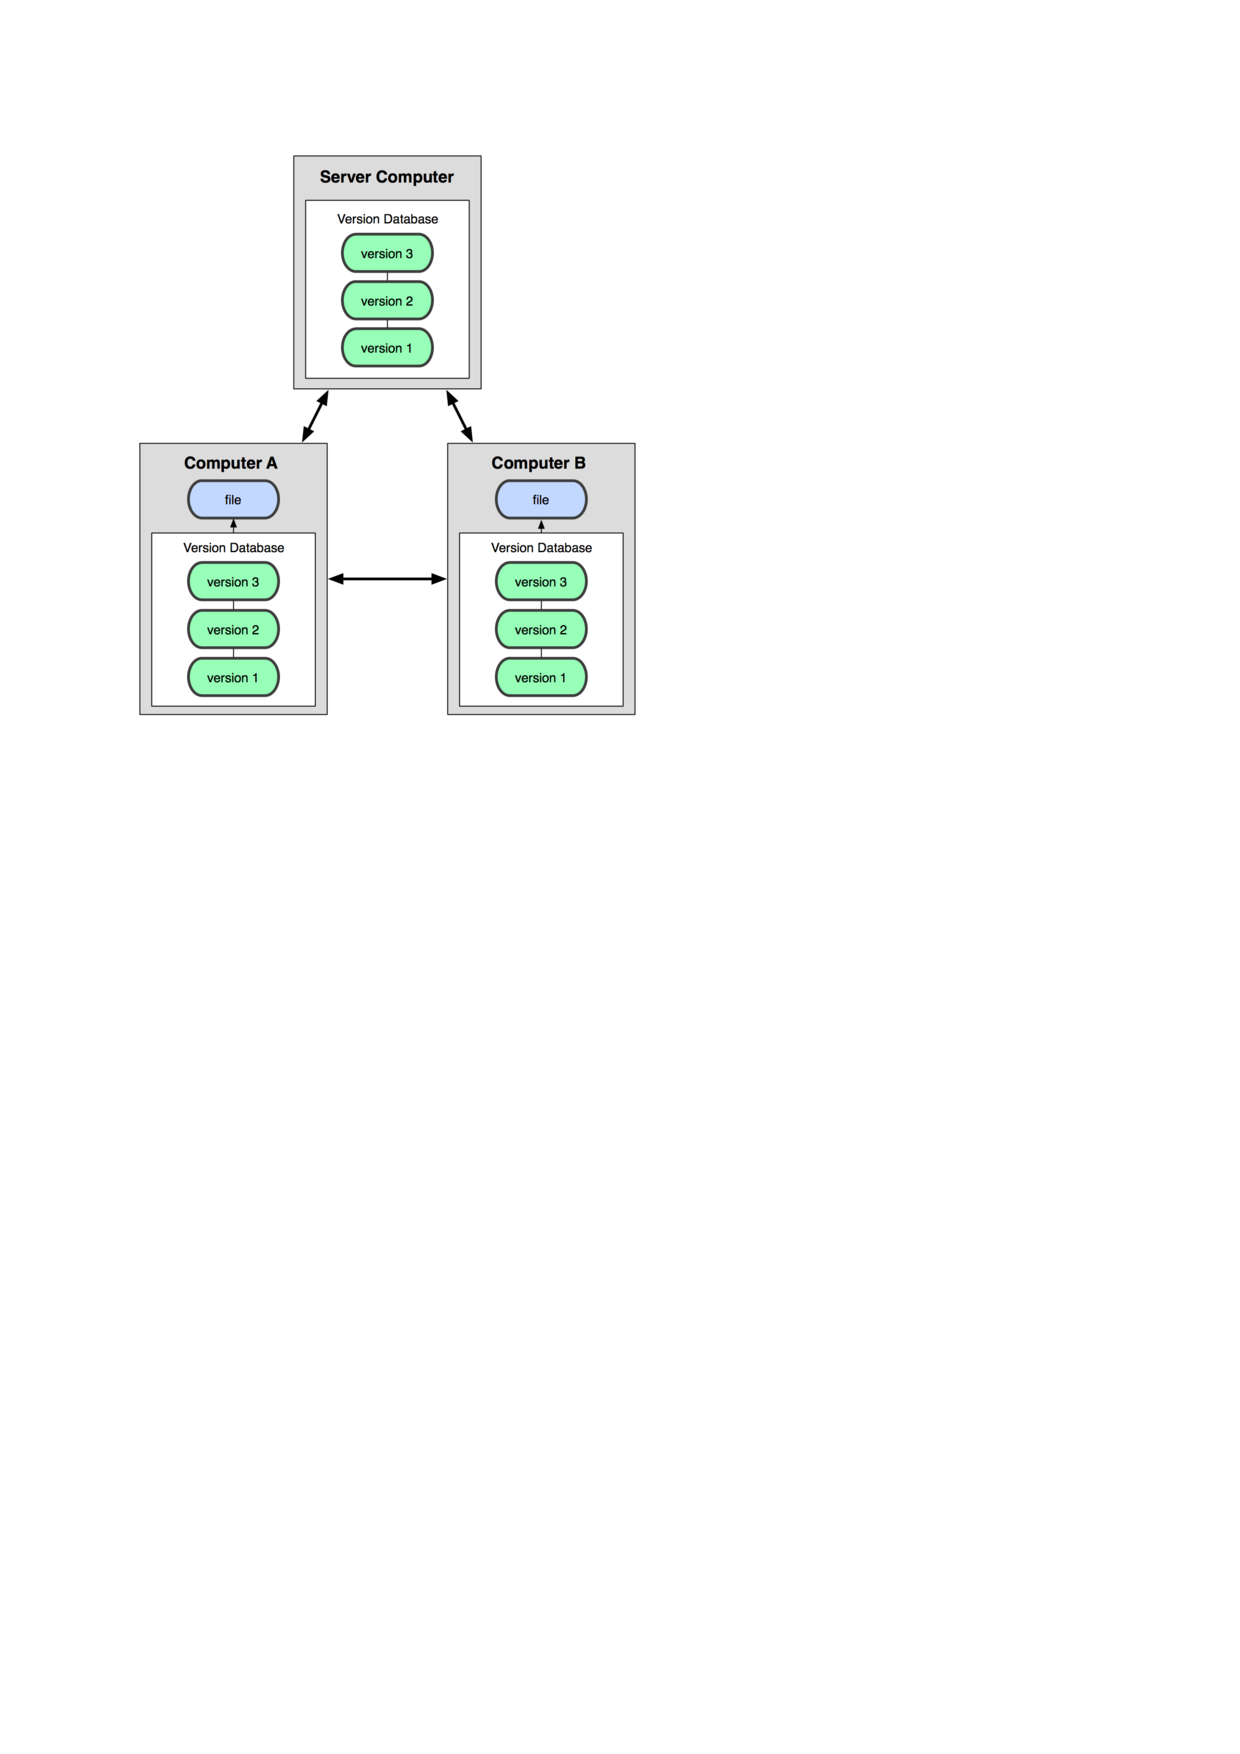
\includegraphics[width=\textwidth]{network}}
\only<2>{
\vspace{3.4cm}
\hspace{0.12cm}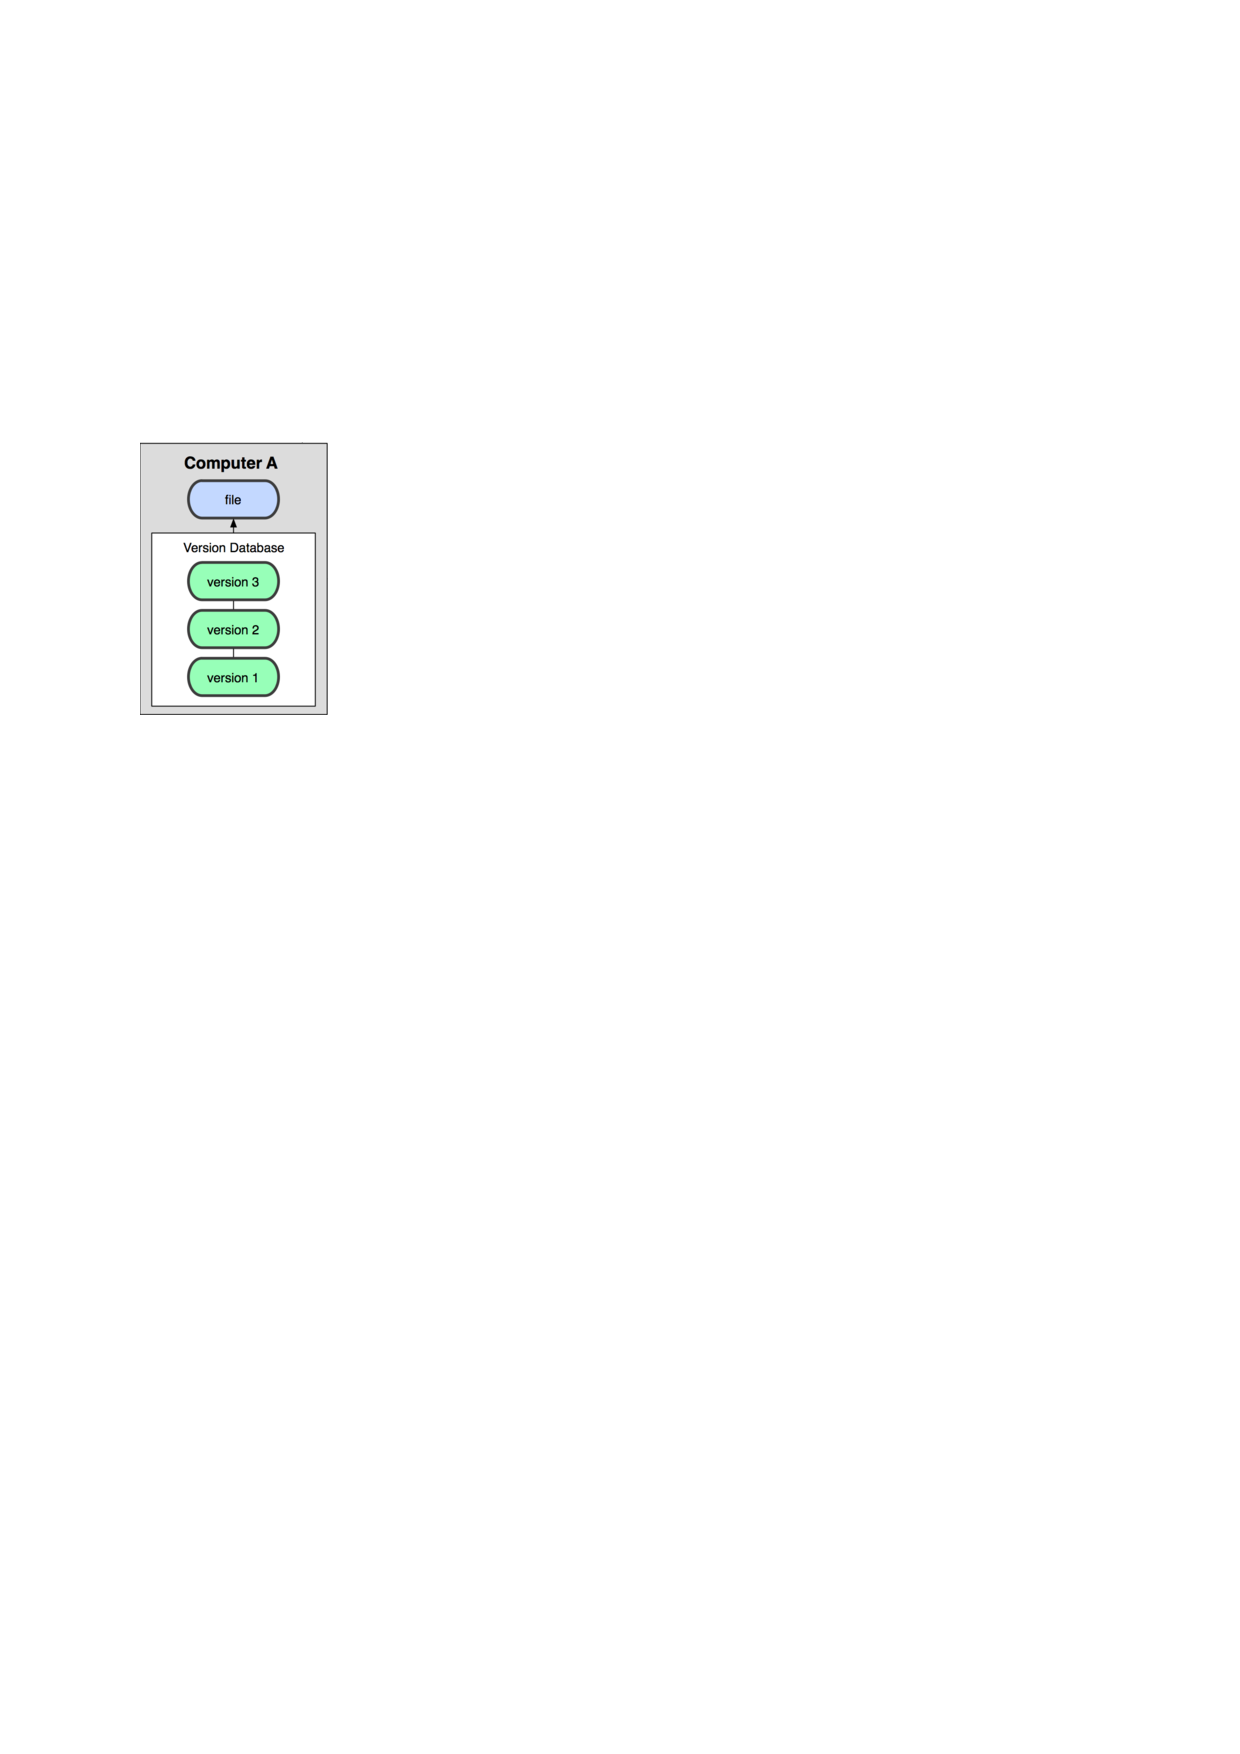
\includegraphics[width=0.365\textwidth]{single_repo}}
\end{minipage}
\begin{minipage}{0.39\textwidth}
\begin{itemize}
\item Version Database: repo/.git~or repo.git\\
\emph{\footnotesize don't got there except if you know what your are doing}
\item Workdir:\\ ``normal" files
\end{itemize}
\end{minipage}
\end{frame}
%%%%%%%%%%%%%%%%%%%%%%%%%%%%%%%%%%%%%%%%
\section{Structure}
\begin{frame}{The structure of the history: the work directory }
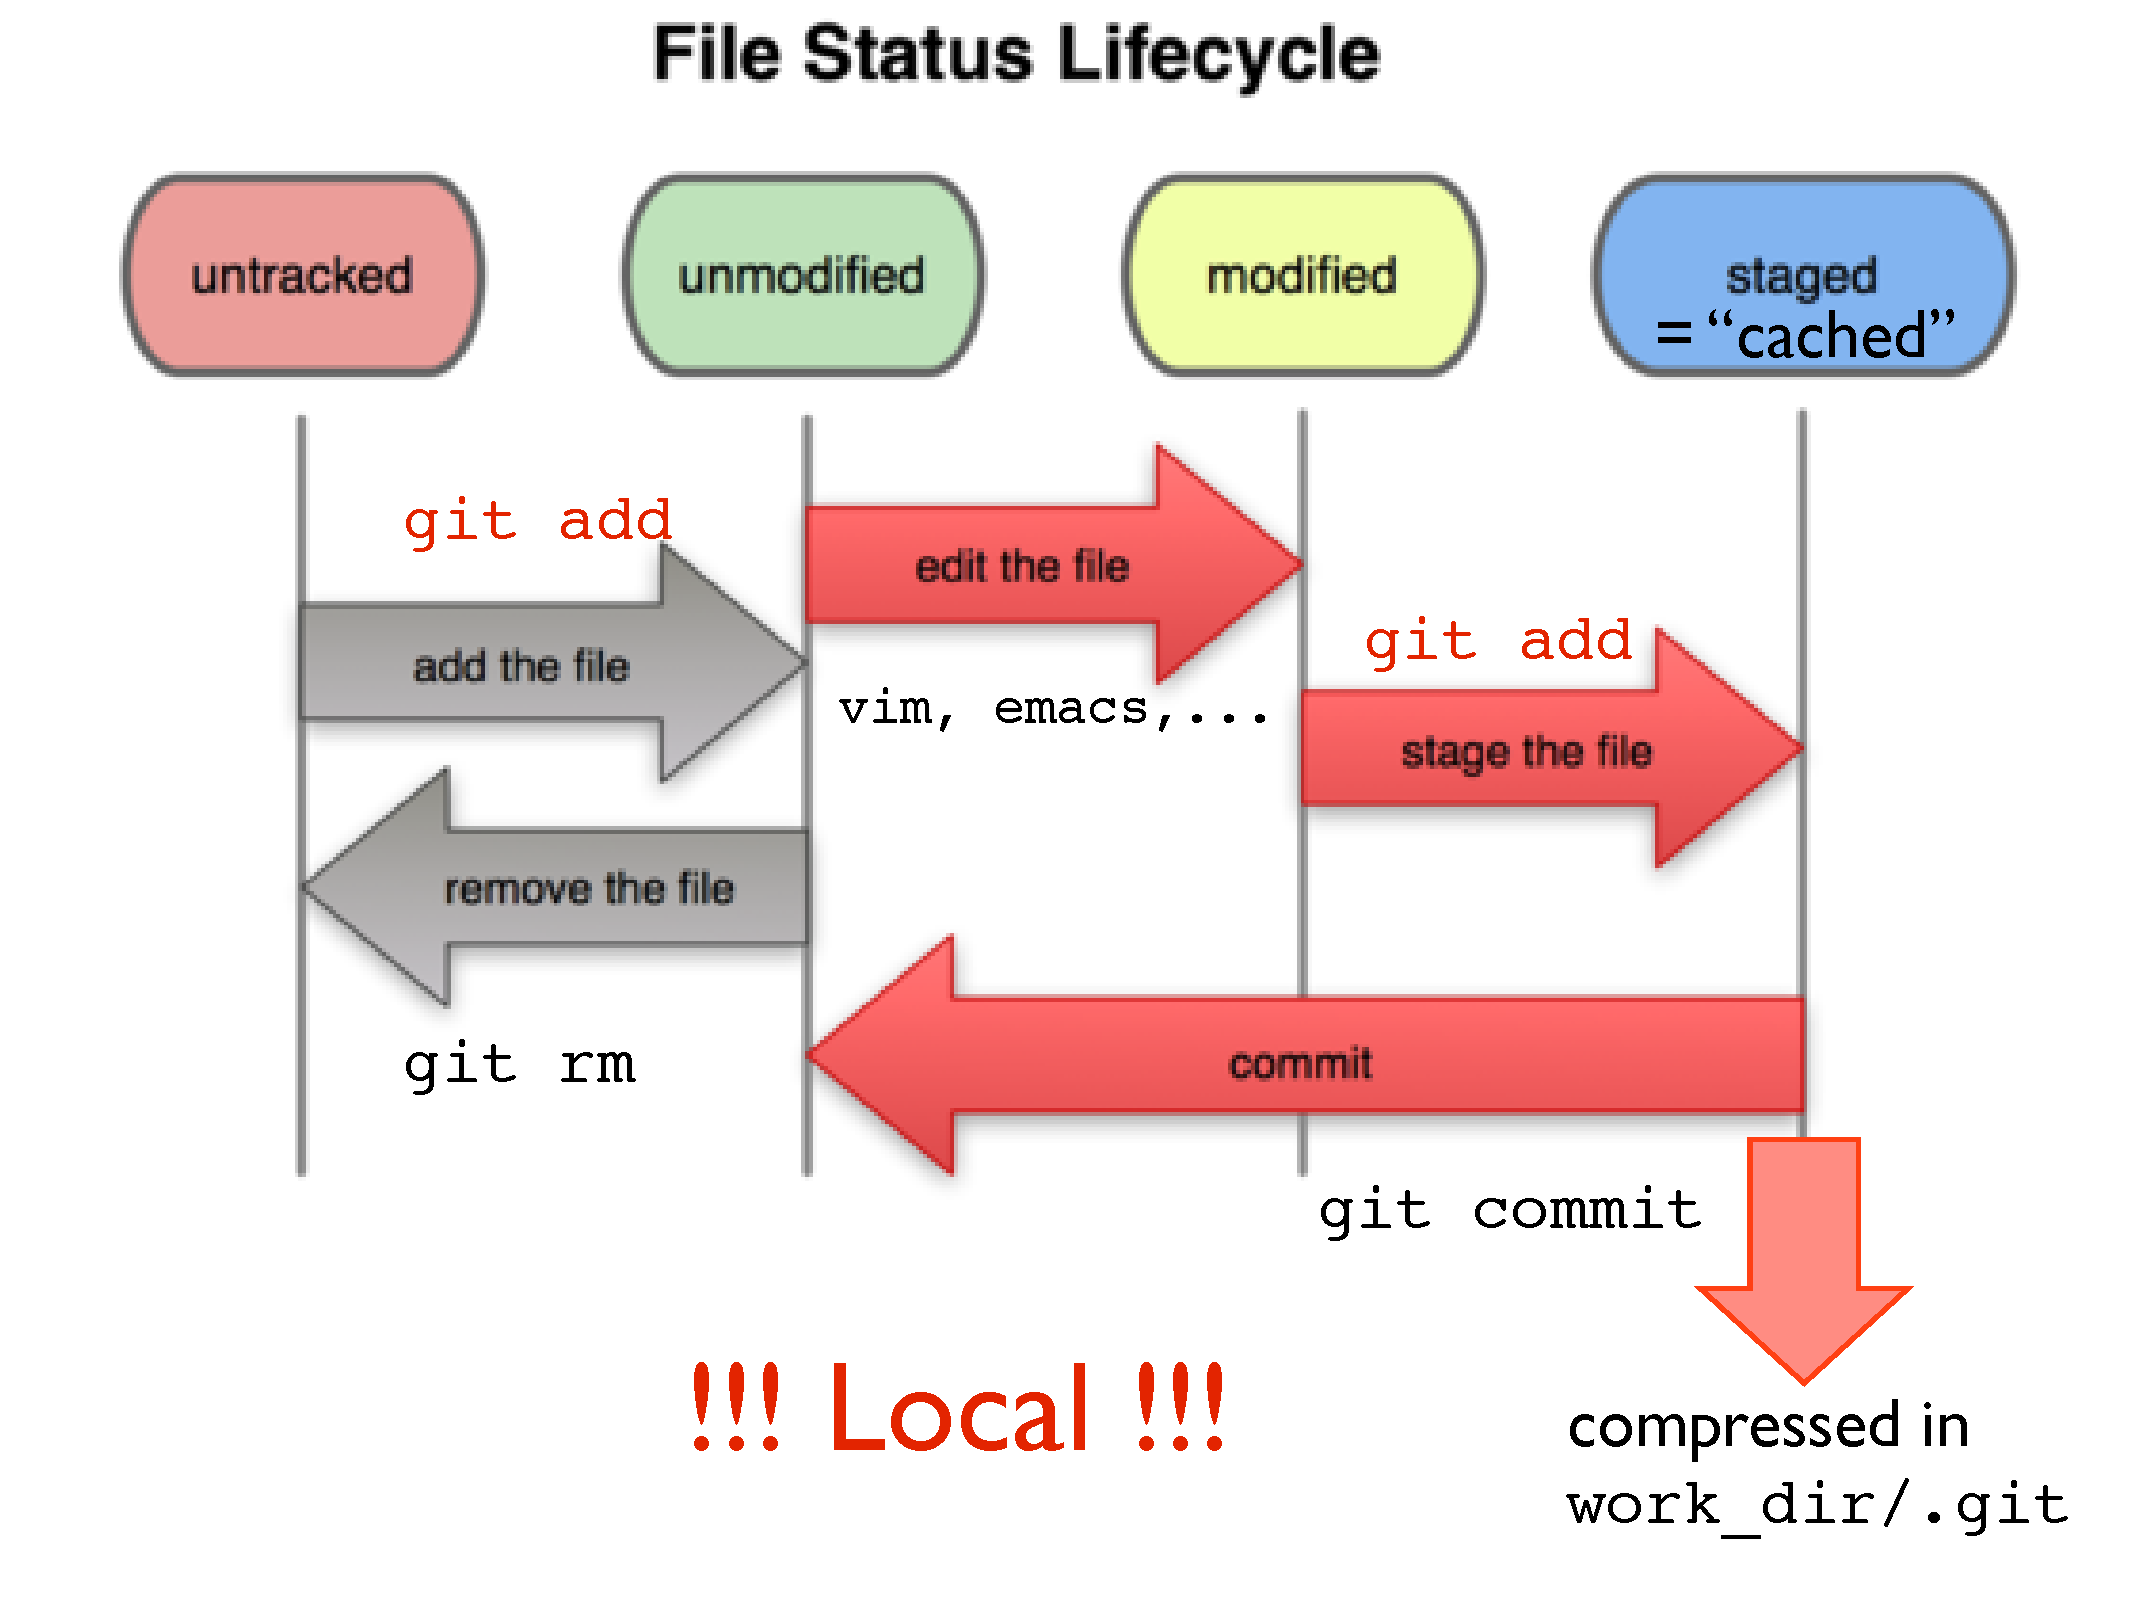
\includegraphics[page=1,width=\textwidth]{local}
\end{frame}
%%%%%%%%%%%%%%%%%%%%
\begin{frame}{The structure of the history: the .git~directory}
\only<1>{\includegraphics[page=2,width=\textwidth]{local}}
\only<2>{\includegraphics[page=3,width=\textwidth]{local}}
\only<3>{\includegraphics[page=4,width=\textwidth]{local}}
\only<4>{\includegraphics[page=5,width=\textwidth]{local}}
\only<5>{\includegraphics[page=6,width=\textwidth]{local}}
\only<6>{\includegraphics[page=7,width=\textwidth]{local}}
\only<7>{\includegraphics[page=8,width=\textwidth]{local}}
\only<8>{\includegraphics[page=9,width=\textwidth]{local}}
\only<9>{\includegraphics[page=10,width=\textwidth]{local}}
\only<10>{\includegraphics[page=11,width=\textwidth]{local}}
\only<11>{\includegraphics[page=12,width=\textwidth]{local}}
\end{frame}
%%%%%%%%%%%%%%%%%%%%
\begin{frame}{Curing panic attacks: reflog and reset}
\only<1>{\includegraphics[page=13,width=\textwidth]{local}}
\only<2>{\includegraphics[page=14,width=\textwidth]{local}}
\only<3>{\includegraphics[page=15,width=\textwidth]{local}}
\end{frame}	
%%%%%%%%%%%%%%%%%%%%
\section{Merging and Collaborating}
\begin{frame}{Merge}
\begin{center}
\begin{color}{red}
\fbox{Merging = combining two \emph{branches} into one}
\end{color}
\end{center}
\begin{block}{\texttt{git~merge <branchName>}}
\begin{itemize}
\item Integrate changes of branchName on the HEAD
\item Conflict resolution in one commit
\item ``nice" way to merge (merged commits stay ancestors)
\end{itemize}
\end{block}\pause
\begin{block}{ \texttt{git~rebase <branchName>} (more advanced) }
\begin{itemize}
\item Replay ancestor commits of HEAD onto branchName
\item Conflict resolutions in each of the new commits
\item old commits become dangling (hopefully)
\item \begin{color}{red}with interactive option: allows to rewrite the history\end{color}
\end{itemize}
\end{block}
\end{frame}
\begin{frame}{Merge}
\begin{center}
\begin{tabular}{rl}
\raisebox{-2.2cm}[1.1cm][0.5cm]{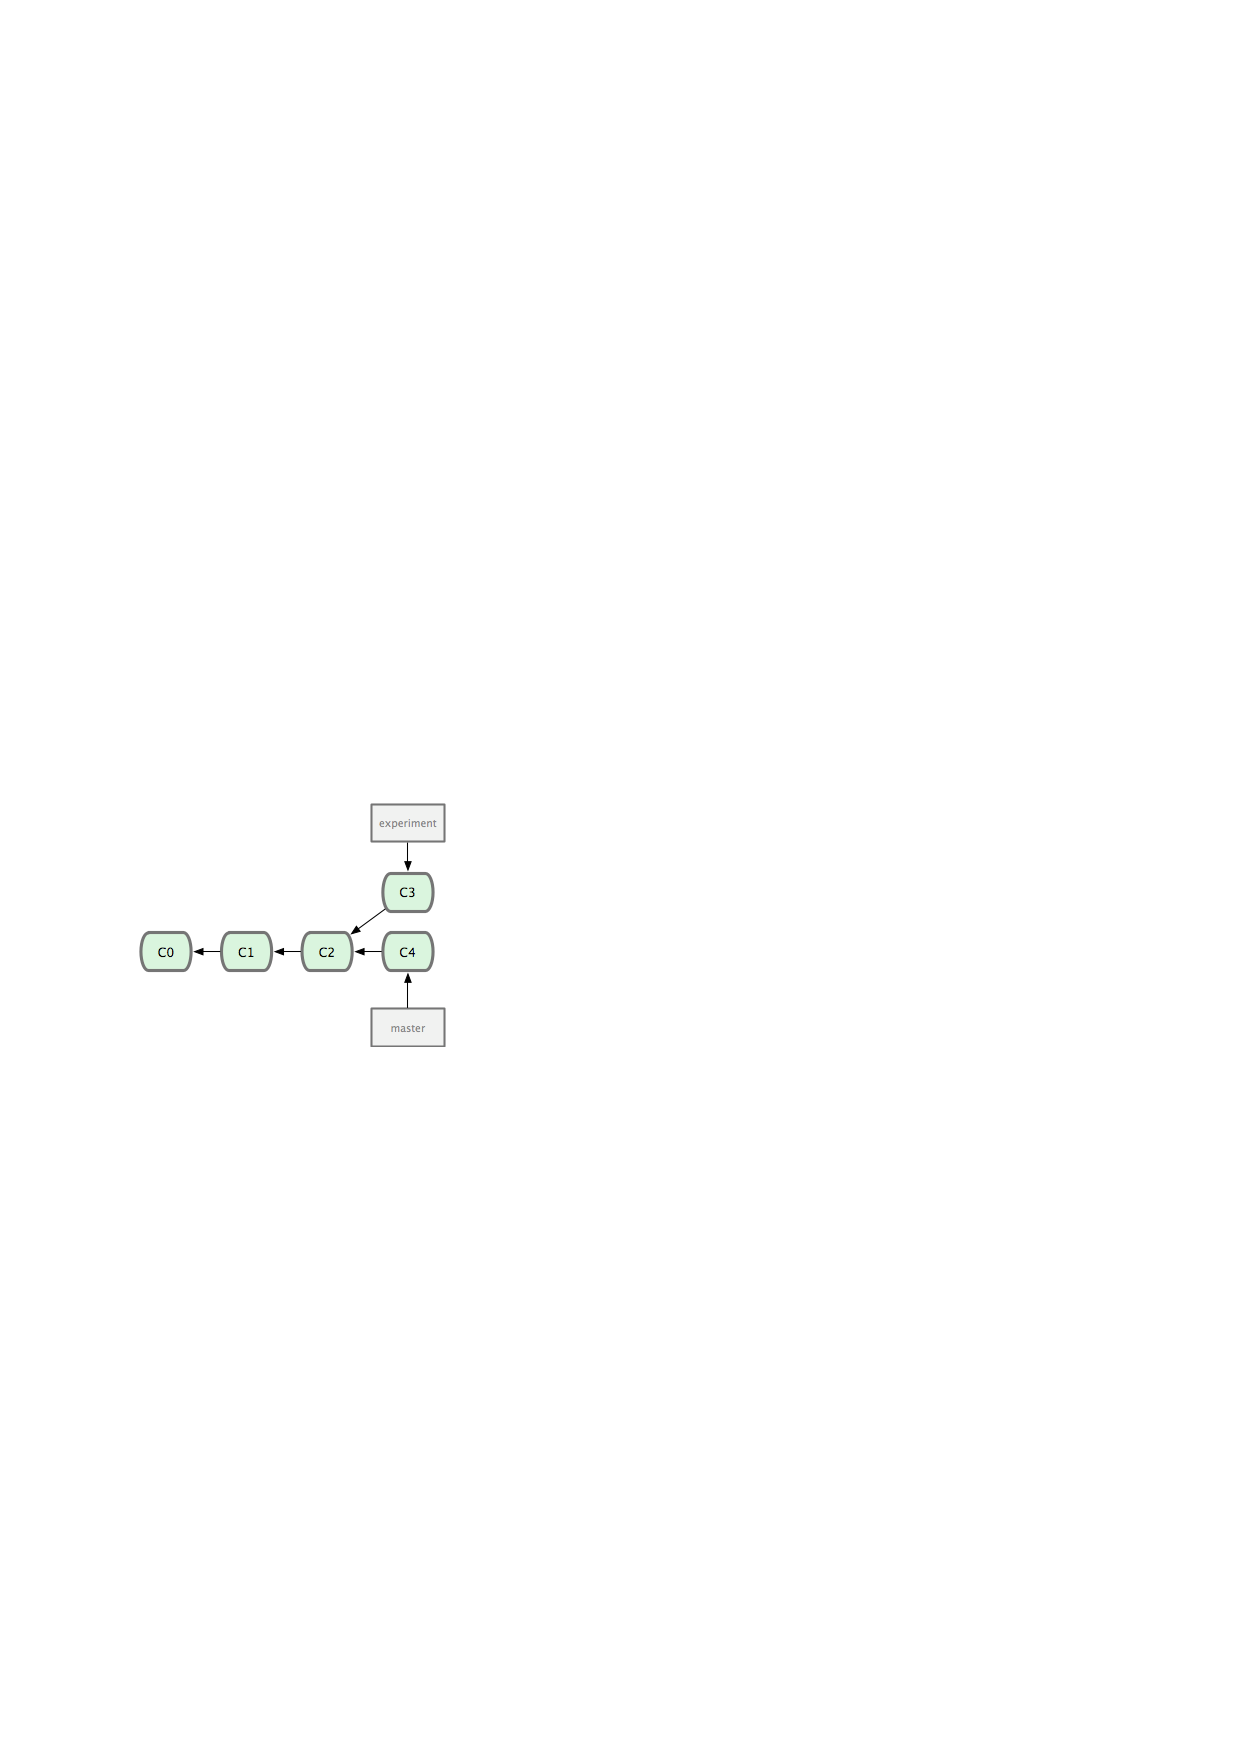
\includegraphics[page=1,width=0.4\textwidth]{merge}}\pause\\
\raisebox{7ex}{\texttt{git~merge:}} & \includegraphics[page=2,width=0.5\textwidth]{merge}\\
\raisebox{7ex}{\texttt{git~rebase:}} & \includegraphics[page=3,width=0.5\textwidth]{merge}\\
\end{tabular}
\end{center}
\end{frame}
%%%%%%%%%%%%%%%%%%%%
\begin{frame}{}
\begin{center}
\only<1>{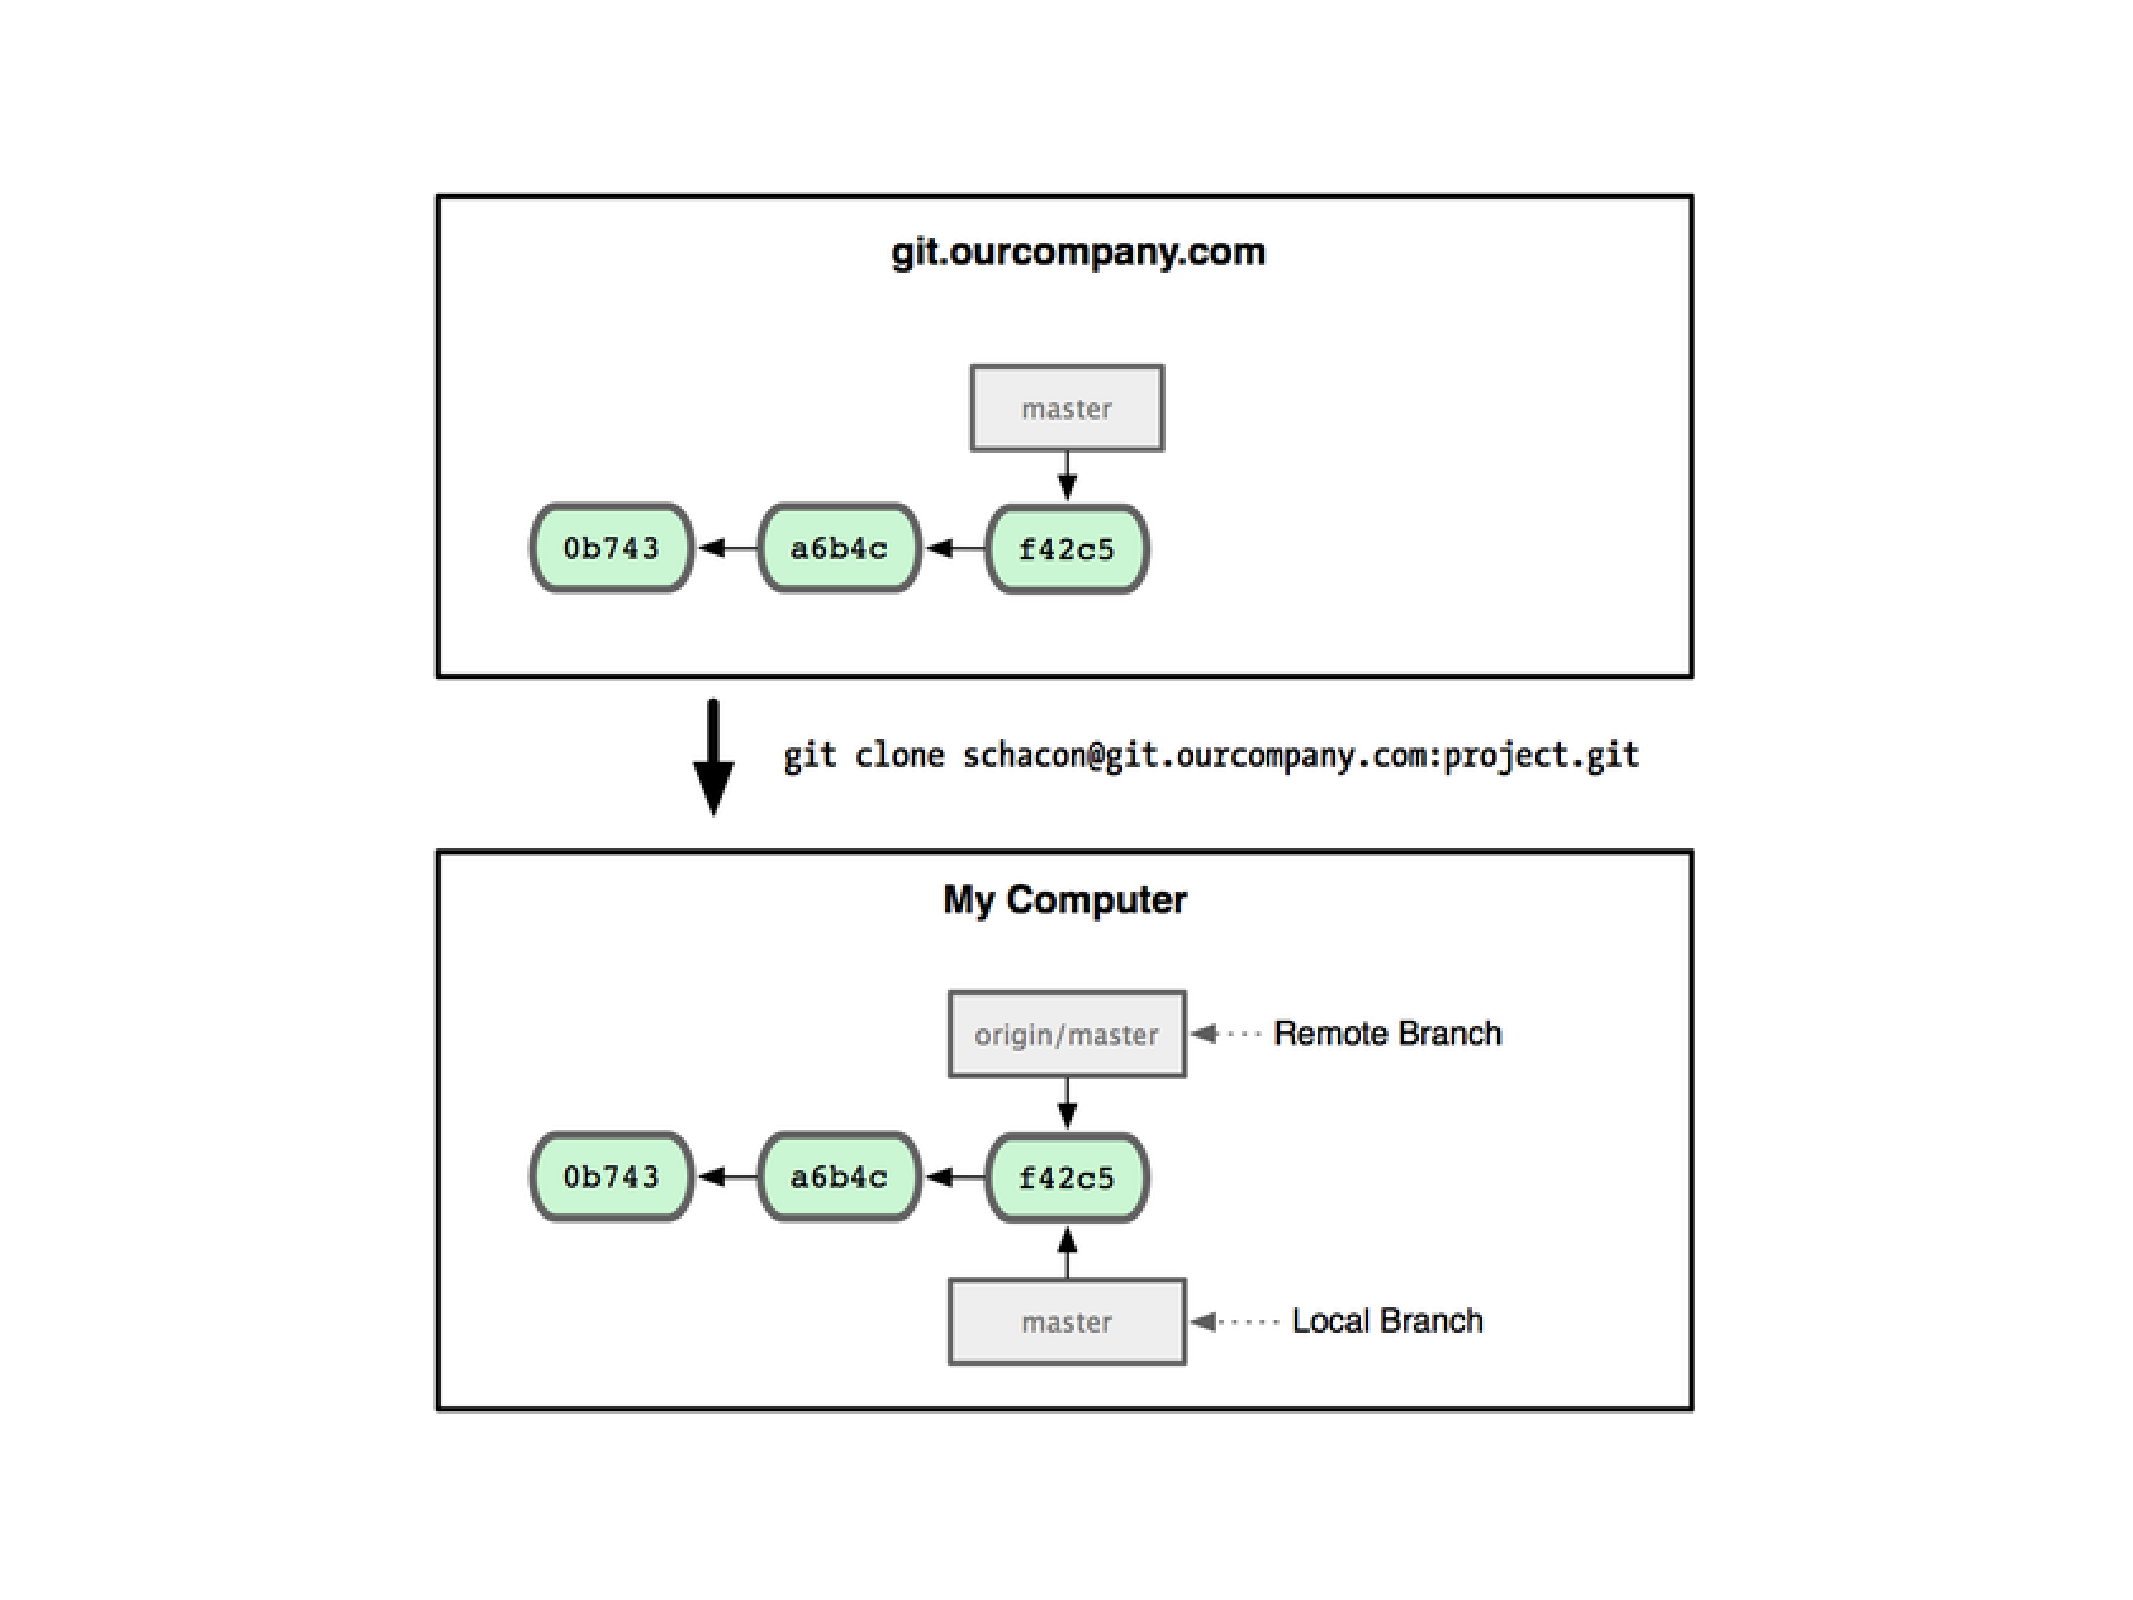
\includegraphics[page=1,width=0.9\textwidth]{withServer}}
\only<2>{\includegraphics[page=2,width=0.9\textwidth]{withServer}}
\only<3->{\includegraphics[page=3,width=0.9\textwidth]{withServer}}
\end{center}
\uncover<4>{more at: \scriptsize \url{http://git-scm.com/book/en/Distributed-Git-Contributing-to-a-Project}}
\end{frame}
%%%%%%%%%%%%%%%%%%%%
\section{Getting started}
\begin{frame}{Getting Started}
\only<1>{\begin{block}{Installation}
System and taste dependent...for installers:
\begin{itemize}
\item linux:  through the built-in package manager
\item mac: \url{http://code.google.com/p/git-osx-installer}
\item window: \url{http://msysgit.github.com/}
\end{itemize}
\end{block}}
\only<2>{
\begin{block}{Configuration: \texttt{git~config}}
\begin{itemize}
\item \texttt{git~config --global user.name "John Doe"}
\item \texttt{git~config --global user.email johndoe@example.com}
\item \begin{color}{red}\texttt{git~config --global core.editor vim -f}\end{color}
\item \begin{color}{red}\texttt{git~config --global merge.tool vim -fd}\end{color}
\end{itemize}
more at: \tiny\url{http://git-scm.com/book/fr/D�marrage-rapide-Param�trage-�-la-premi�re-utilisation-de-Git}

\end{block}}
\end{frame}
\begin{frame}{Getting Started: from scratch}
Please enter a directory that you want to monitor with git\pause
\begin{block}{Working with git}
\begin{itemize}
\item Create a repo: \texttt{git~init}\pause
\item Edit .gitignore\pause
\item Work within a repo: \texttt{git~add}, \texttt{git~commit}, \texttt{git~branch}, etc.\pause
\item See info about a repo: \texttt{git~status}, \texttt{git~diff},\\ \texttt{git~log}, \texttt{git~reflog}, etc.\pause
\item Work with others: \texttt{git~pull}, \texttt{git~push}, \texttt{git~fetch},
 \texttt{git~remote},
 etc. \pause
\item Getting help: \texttt{git~[<cmd>] help}
\end{itemize}
\end{block}
\end{frame}

\begin{frame}{Getting started on an existing project}
Please enter a directory where you want to save the seminar material\pause
\begin{block}{}
\texttt{\footnotesize git~clone \url{https://github.com/tcarette/gitSeminar.git}}
\end{block}
\end{frame}
%%%%%%%%%%%%%%%%%%%%
\section{Additional Resources}
\begin{frame}{URLs}
\tiny

\begin{block}{References}
\url{http://git-scm.com/} (Official website)\\
\url{http://git-scm.com/book} (Pro git)
\end{block}

\begin{block}{Cheat sheets}
\url{http://www.git-tower.com/blog/git-cheat-sheet/}\\
\url{http://ndpsoftware.com/git-cheatsheet.html}
\end{block}

\begin{block}{Graphical User Interface (GUI)}
\url{http://git-scm.com/downloads/guis}\\
\url{http://www.sourcetreeapp.com/} (the one I use)
\end{block}

\begin{block}{Free git~servers}
\url{https://github.com/} (good for open/public repositories)\\
\url{https://bitbucket.org/} (good for private repositories)
\end{block}

\begin{block}{Other}
\url{http://blog.vogella.com/2013/03/19/git-auto-completion-for-the-bash-shell/} (autocomplete)\\
\url{https://help.github.com/articles/generating-ssh-keys} (ssh keys)
%\url{http://fuse.sourceforge.net/sshfs.html} (mount remote directories. mac: on homebrew, windows: \url{http://linhost.info/2012/09/sshfs-in-windows/})
\end{block}

\end{frame}
\end{document}
